\documentclass[twoside]{book}

% Packages required by doxygen
\usepackage{fixltx2e}
\usepackage{calc}
\usepackage{doxygen}
\usepackage[export]{adjustbox} % also loads graphicx
\usepackage{graphicx}
\usepackage[utf8]{inputenc}
\usepackage{makeidx}
\usepackage{multicol}
\usepackage{multirow}
\PassOptionsToPackage{warn}{textcomp}
\usepackage{textcomp}
\usepackage[nointegrals]{wasysym}
\usepackage[table]{xcolor}

% Font selection
\usepackage[T1]{fontenc}
\usepackage[scaled=.90]{helvet}
\usepackage{courier}
\usepackage{amssymb}
\usepackage{sectsty}
\renewcommand{\familydefault}{\sfdefault}
\allsectionsfont{%
  \fontseries{bc}\selectfont%
  \color{darkgray}%
}
\renewcommand{\DoxyLabelFont}{%
  \fontseries{bc}\selectfont%
  \color{darkgray}%
}
\newcommand{\+}{\discretionary{\mbox{\scriptsize$\hookleftarrow$}}{}{}}

% Page & text layout
\usepackage{geometry}
\geometry{%
  a4paper,%
  top=2.5cm,%
  bottom=2.5cm,%
  left=2.5cm,%
  right=2.5cm%
}
\tolerance=750
\hfuzz=15pt
\hbadness=750
\setlength{\emergencystretch}{15pt}
\setlength{\parindent}{0cm}
\setlength{\parskip}{3ex plus 2ex minus 2ex}
\makeatletter
\renewcommand{\paragraph}{%
  \@startsection{paragraph}{4}{0ex}{-1.0ex}{1.0ex}{%
    \normalfont\normalsize\bfseries\SS@parafont%
  }%
}
\renewcommand{\subparagraph}{%
  \@startsection{subparagraph}{5}{0ex}{-1.0ex}{1.0ex}{%
    \normalfont\normalsize\bfseries\SS@subparafont%
  }%
}
\makeatother

% Headers & footers
\usepackage{fancyhdr}
\pagestyle{fancyplain}
\fancyhead[LE]{\fancyplain{}{\bfseries\thepage}}
\fancyhead[CE]{\fancyplain{}{}}
\fancyhead[RE]{\fancyplain{}{\bfseries\leftmark}}
\fancyhead[LO]{\fancyplain{}{\bfseries\rightmark}}
\fancyhead[CO]{\fancyplain{}{}}
\fancyhead[RO]{\fancyplain{}{\bfseries\thepage}}
\fancyfoot[LE]{\fancyplain{}{}}
\fancyfoot[CE]{\fancyplain{}{}}
\fancyfoot[RE]{\fancyplain{}{\bfseries\scriptsize Generated by Doxygen }}
\fancyfoot[LO]{\fancyplain{}{\bfseries\scriptsize Generated by Doxygen }}
\fancyfoot[CO]{\fancyplain{}{}}
\fancyfoot[RO]{\fancyplain{}{}}
\renewcommand{\footrulewidth}{0.4pt}
\renewcommand{\chaptermark}[1]{%
  \markboth{#1}{}%
}
\renewcommand{\sectionmark}[1]{%
  \markright{\thesection\ #1}%
}

% Indices & bibliography
\usepackage{natbib}
\usepackage[titles]{tocloft}
\setcounter{tocdepth}{3}
\setcounter{secnumdepth}{5}
\makeindex

% Hyperlinks (required, but should be loaded last)
\usepackage{ifpdf}
\ifpdf
  \usepackage[pdftex,pagebackref=true]{hyperref}
\else
  \usepackage[ps2pdf,pagebackref=true]{hyperref}
\fi
\hypersetup{%
  colorlinks=true,%
  linkcolor=blue,%
  citecolor=blue,%
  unicode%
}

% Custom commands
\newcommand{\clearemptydoublepage}{%
  \newpage{\pagestyle{empty}\cleardoublepage}%
}

\usepackage{caption}
\captionsetup{labelsep=space,justification=centering,font={bf},singlelinecheck=off,skip=4pt,position=top}

%===== C O N T E N T S =====

\begin{document}

% Titlepage & ToC
\hypersetup{pageanchor=false,
             bookmarksnumbered=true,
             pdfencoding=unicode
            }
\pagenumbering{alph}
\begin{titlepage}
\vspace*{7cm}
\begin{center}%
{\Large My Project \\[1ex]\large 1.\+0 }\\
\vspace*{1cm}
{\large Generated by Doxygen 1.8.14}\\
\end{center}
\end{titlepage}
\clearemptydoublepage
\pagenumbering{roman}
\tableofcontents
\clearemptydoublepage
\pagenumbering{arabic}
\hypersetup{pageanchor=true}

%--- Begin generated contents ---
\chapter{Hierarchical Index}
\section{Class Hierarchy}
This inheritance list is sorted roughly, but not completely, alphabetically\+:\begin{DoxyCompactList}
\item \contentsline{section}{B\+OY}{\pageref{classBOY}}{}
\begin{DoxyCompactList}
\item \contentsline{section}{G\+E\+E\+KS}{\pageref{classGEEKS}}{}
\item \contentsline{section}{G\+E\+N\+E\+R\+O\+US}{\pageref{classGENEROUS}}{}
\item \contentsline{section}{M\+I\+S\+ER}{\pageref{classMISER}}{}
\end{DoxyCompactList}
\item \contentsline{section}{couple}{\pageref{structcouple}}{}
\item \contentsline{section}{G\+I\+FT}{\pageref{classGIFT}}{}
\item \contentsline{section}{G\+I\+RL}{\pageref{classGIRL}}{}
\begin{DoxyCompactList}
\item \contentsline{section}{C\+H\+O\+O\+SY}{\pageref{classCHOOSY}}{}
\item \contentsline{section}{D\+E\+S\+P\+E\+R\+A\+TE}{\pageref{classDESPERATE}}{}
\end{DoxyCompactList}
\end{DoxyCompactList}

\chapter{Class Index}
\section{Class List}
Here are the classes, structs, unions and interfaces with brief descriptions\+:\begin{DoxyCompactList}
\item\contentsline{section}{\hyperlink{classBOY}{B\+OY} \\*Class name \hyperlink{classBOY}{B\+OY} }{\pageref{classBOY}}{}
\item\contentsline{section}{\hyperlink{classCHOOSY}{C\+H\+O\+O\+SY} }{\pageref{classCHOOSY}}{}
\item\contentsline{section}{\hyperlink{structcouple}{couple} }{\pageref{structcouple}}{}
\item\contentsline{section}{\hyperlink{classDESPERATE}{D\+E\+S\+P\+E\+R\+A\+TE} }{\pageref{classDESPERATE}}{}
\item\contentsline{section}{\hyperlink{classGEEKS}{G\+E\+E\+KS} }{\pageref{classGEEKS}}{}
\item\contentsline{section}{\hyperlink{classGENEROUS}{G\+E\+N\+E\+R\+O\+US} \\*Class name \hyperlink{classGENEROUS}{G\+E\+N\+E\+R\+O\+US} }{\pageref{classGENEROUS}}{}
\item\contentsline{section}{\hyperlink{classGIFT}{G\+I\+FT} }{\pageref{classGIFT}}{}
\item\contentsline{section}{\hyperlink{classGIRL}{G\+I\+RL} }{\pageref{classGIRL}}{}
\item\contentsline{section}{\hyperlink{classMISER}{M\+I\+S\+ER} }{\pageref{classMISER}}{}
\end{DoxyCompactList}

\chapter{Class Documentation}
\hypertarget{classBOY}{}\section{B\+OY Class Reference}
\label{classBOY}\index{B\+OY@{B\+OY}}


class name \hyperlink{classBOY}{B\+OY}  




{\ttfamily \#include $<$B\+O\+Y.\+h$>$}

Inheritance diagram for B\+OY\+:\begin{figure}[H]
\begin{center}
\leavevmode
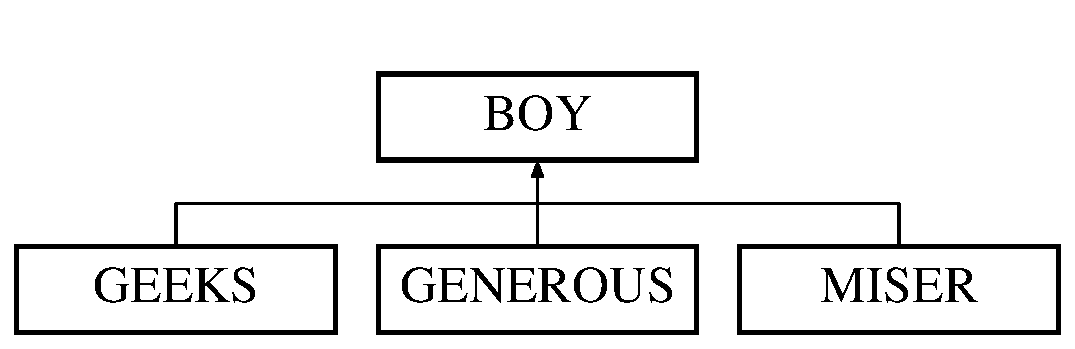
\includegraphics[height=2.000000cm]{classBOY}
\end{center}
\end{figure}
\subsection*{Public Attributes}
\begin{DoxyCompactItemize}
\item 
\mbox{\Hypertarget{classBOY_abf715bd190db0239dd44791d53458b34}\label{classBOY_abf715bd190db0239dd44791d53458b34}} 
char {\bfseries name} \mbox{[}10\mbox{]}
\item 
\mbox{\Hypertarget{classBOY_ae0412607bcd68ca79cb0eb4715f1a9bc}\label{classBOY_ae0412607bcd68ca79cb0eb4715f1a9bc}} 
int \hyperlink{classBOY_ae0412607bcd68ca79cb0eb4715f1a9bc}{attract}
\begin{DoxyCompactList}\small\item\em name of boy \end{DoxyCompactList}\item 
\mbox{\Hypertarget{classBOY_a0b17a61e6d1c032b638cef05192a2a38}\label{classBOY_a0b17a61e6d1c032b638cef05192a2a38}} 
int \hyperlink{classBOY_a0b17a61e6d1c032b638cef05192a2a38}{budget}
\begin{DoxyCompactList}\small\item\em attractiveness \end{DoxyCompactList}\item 
\mbox{\Hypertarget{classBOY_afbb490388a031bea3e62c561d03ee525}\label{classBOY_afbb490388a031bea3e62c561d03ee525}} 
int {\bfseries int\+\_\+level}
\item 
\mbox{\Hypertarget{classBOY_aca986517df0bc12d682203faae7bc59f}\label{classBOY_aca986517df0bc12d682203faae7bc59f}} 
char \hyperlink{classBOY_aca986517df0bc12d682203faae7bc59f}{type} \mbox{[}10\mbox{]}
\begin{DoxyCompactList}\small\item\em status \end{DoxyCompactList}\item 
\mbox{\Hypertarget{classBOY_a3b7d109c795e1cf488166b7436411586}\label{classBOY_a3b7d109c795e1cf488166b7436411586}} 
double {\bfseries happ}
\item 
\mbox{\Hypertarget{classBOY_a3060f1f55150949d15a3889e49fda6b3}\label{classBOY_a3060f1f55150949d15a3889e49fda6b3}} 
char \hyperlink{classBOY_a3060f1f55150949d15a3889e49fda6b3}{status} \mbox{[}10\mbox{]}
\begin{DoxyCompactList}\small\item\em happiness \end{DoxyCompactList}\end{DoxyCompactItemize}


\subsection{Detailed Description}
class name \hyperlink{classBOY}{B\+OY} 

The documentation for this class was generated from the following files\+:\begin{DoxyCompactItemize}
\item 
ppl\+Q2.\+cpp\item 
B\+O\+Y.\+h\end{DoxyCompactItemize}

\hypertarget{classCHOOSY}{}\section{C\+H\+O\+O\+SY Class Reference}
\label{classCHOOSY}\index{C\+H\+O\+O\+SY@{C\+H\+O\+O\+SY}}
Inheritance diagram for C\+H\+O\+O\+SY\+:\begin{figure}[H]
\begin{center}
\leavevmode
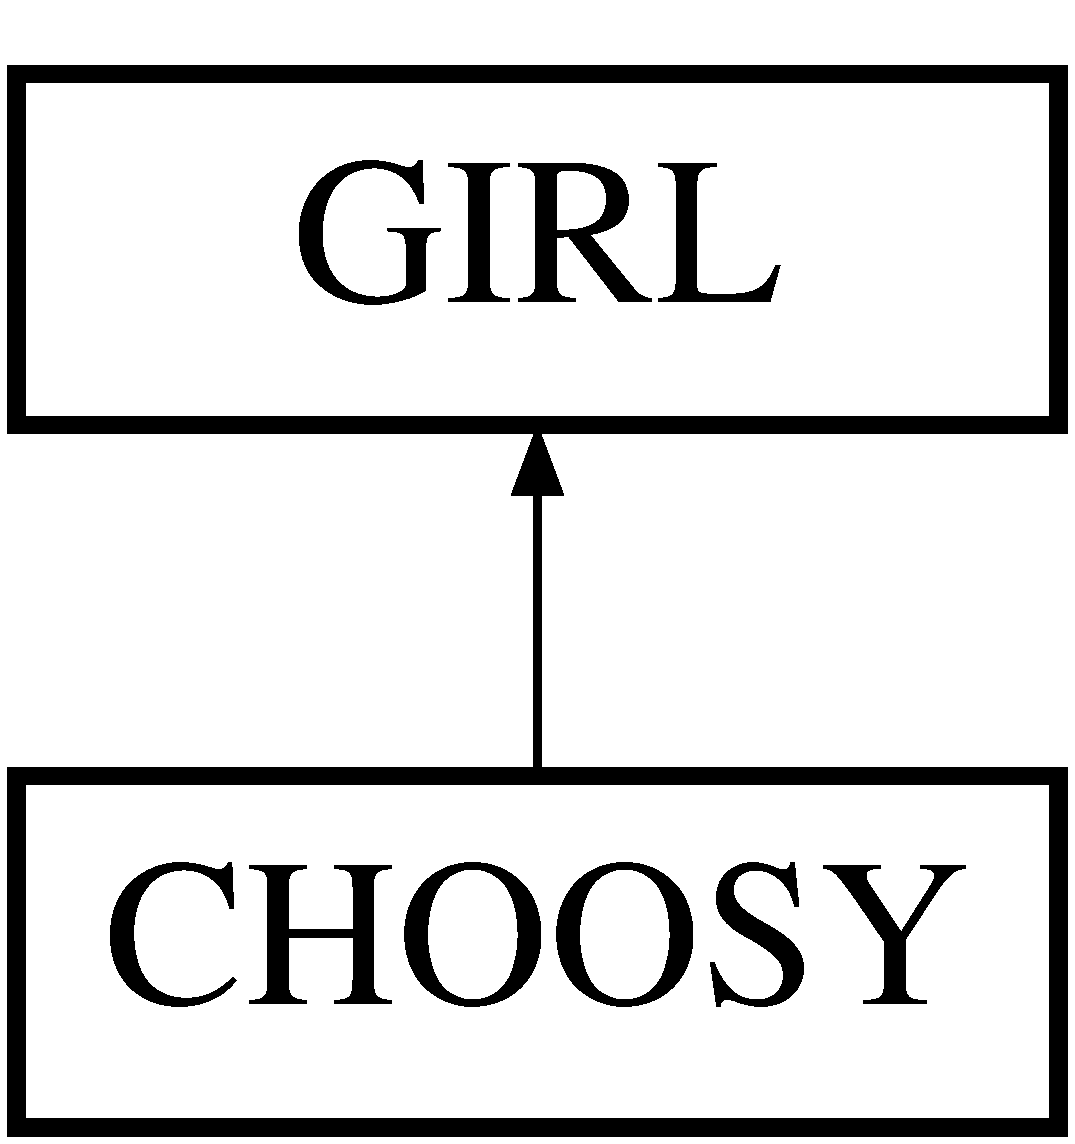
\includegraphics[height=2.000000cm]{classCHOOSY}
\end{center}
\end{figure}
\subsection*{Public Member Functions}
\begin{DoxyCompactItemize}
\item 
\mbox{\Hypertarget{classCHOOSY_a002ab00256ec849228b25d95dd4e0526}\label{classCHOOSY_a002ab00256ec849228b25d95dd4e0526}} 
double \hyperlink{classCHOOSY_a002ab00256ec849228b25d95dd4e0526}{cal\+\_\+happ} (int gift\+\_\+price, int gift\+\_\+value)
\begin{DoxyCompactList}\small\item\em child class of \hyperlink{classGIRL}{G\+I\+RL} class \end{DoxyCompactList}\end{DoxyCompactItemize}
\subsection*{Additional Inherited Members}


The documentation for this class was generated from the following file\+:\begin{DoxyCompactItemize}
\item 
C\+H\+O\+O\+S\+Y.\+h\end{DoxyCompactItemize}

\hypertarget{structcouple}{}\section{couple Struct Reference}
\label{structcouple}\index{couple@{couple}}
\subsection*{Public Attributes}
\begin{DoxyCompactItemize}
\item 
\mbox{\Hypertarget{structcouple_a9d1fb6b20757287852e7bedb702c32f7}\label{structcouple_a9d1fb6b20757287852e7bedb702c32f7}} 
char {\bfseries name1} \mbox{[}10\mbox{]}
\item 
\mbox{\Hypertarget{structcouple_af556c7451b28974deefa0f995b9e7f99}\label{structcouple_af556c7451b28974deefa0f995b9e7f99}} 
char {\bfseries name2} \mbox{[}10\mbox{]}
\item 
\mbox{\Hypertarget{structcouple_a6cdd0405460995565bcae32f66cd8b74}\label{structcouple_a6cdd0405460995565bcae32f66cd8b74}} 
int {\bfseries comp}
\end{DoxyCompactItemize}


The documentation for this struct was generated from the following file\+:\begin{DoxyCompactItemize}
\item 
F\+I\+N\+D\+\_\+\+G\+F1.\+h\end{DoxyCompactItemize}

\hypertarget{classDESPERATE}{}\section{D\+E\+S\+P\+E\+R\+A\+TE Class Reference}
\label{classDESPERATE}\index{D\+E\+S\+P\+E\+R\+A\+TE@{D\+E\+S\+P\+E\+R\+A\+TE}}
Inheritance diagram for D\+E\+S\+P\+E\+R\+A\+TE\+:\begin{figure}[H]
\begin{center}
\leavevmode
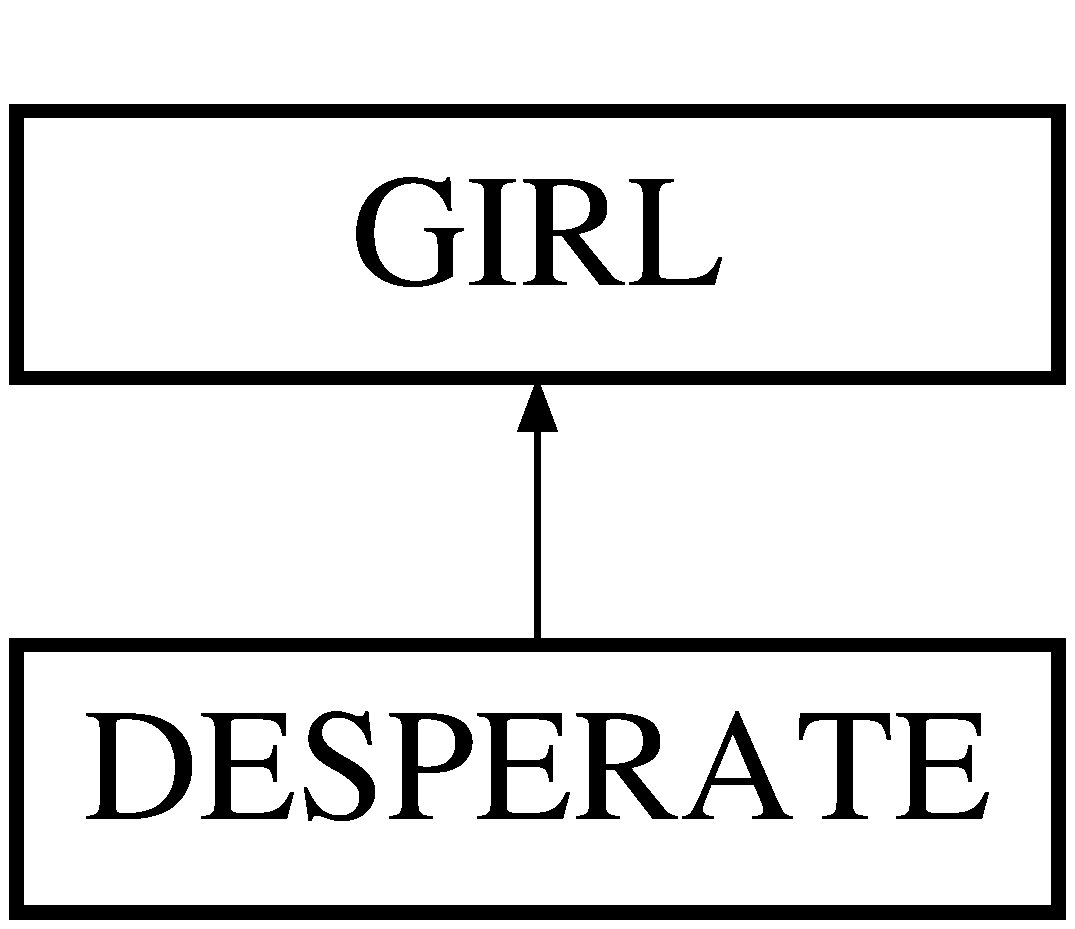
\includegraphics[height=2.000000cm]{classDESPERATE}
\end{center}
\end{figure}
\subsection*{Public Member Functions}
\begin{DoxyCompactItemize}
\item 
\mbox{\Hypertarget{classDESPERATE_a45cf54b78a2087c6935118bf4ba3f80b}\label{classDESPERATE_a45cf54b78a2087c6935118bf4ba3f80b}} 
double \hyperlink{classDESPERATE_a45cf54b78a2087c6935118bf4ba3f80b}{cal\+\_\+happ} (int gift\+\_\+price, int gift\+\_\+value)
\begin{DoxyCompactList}\small\item\em child class of \hyperlink{classGIRL}{G\+I\+RL} class \end{DoxyCompactList}\end{DoxyCompactItemize}
\subsection*{Additional Inherited Members}


The documentation for this class was generated from the following file\+:\begin{DoxyCompactItemize}
\item 
D\+E\+S\+P\+E\+R\+A\+T\+E.\+h\end{DoxyCompactItemize}

\hypertarget{classGEEKS}{}\section{G\+E\+E\+KS Class Reference}
\label{classGEEKS}\index{G\+E\+E\+KS@{G\+E\+E\+KS}}
Inheritance diagram for G\+E\+E\+KS\+:\begin{figure}[H]
\begin{center}
\leavevmode
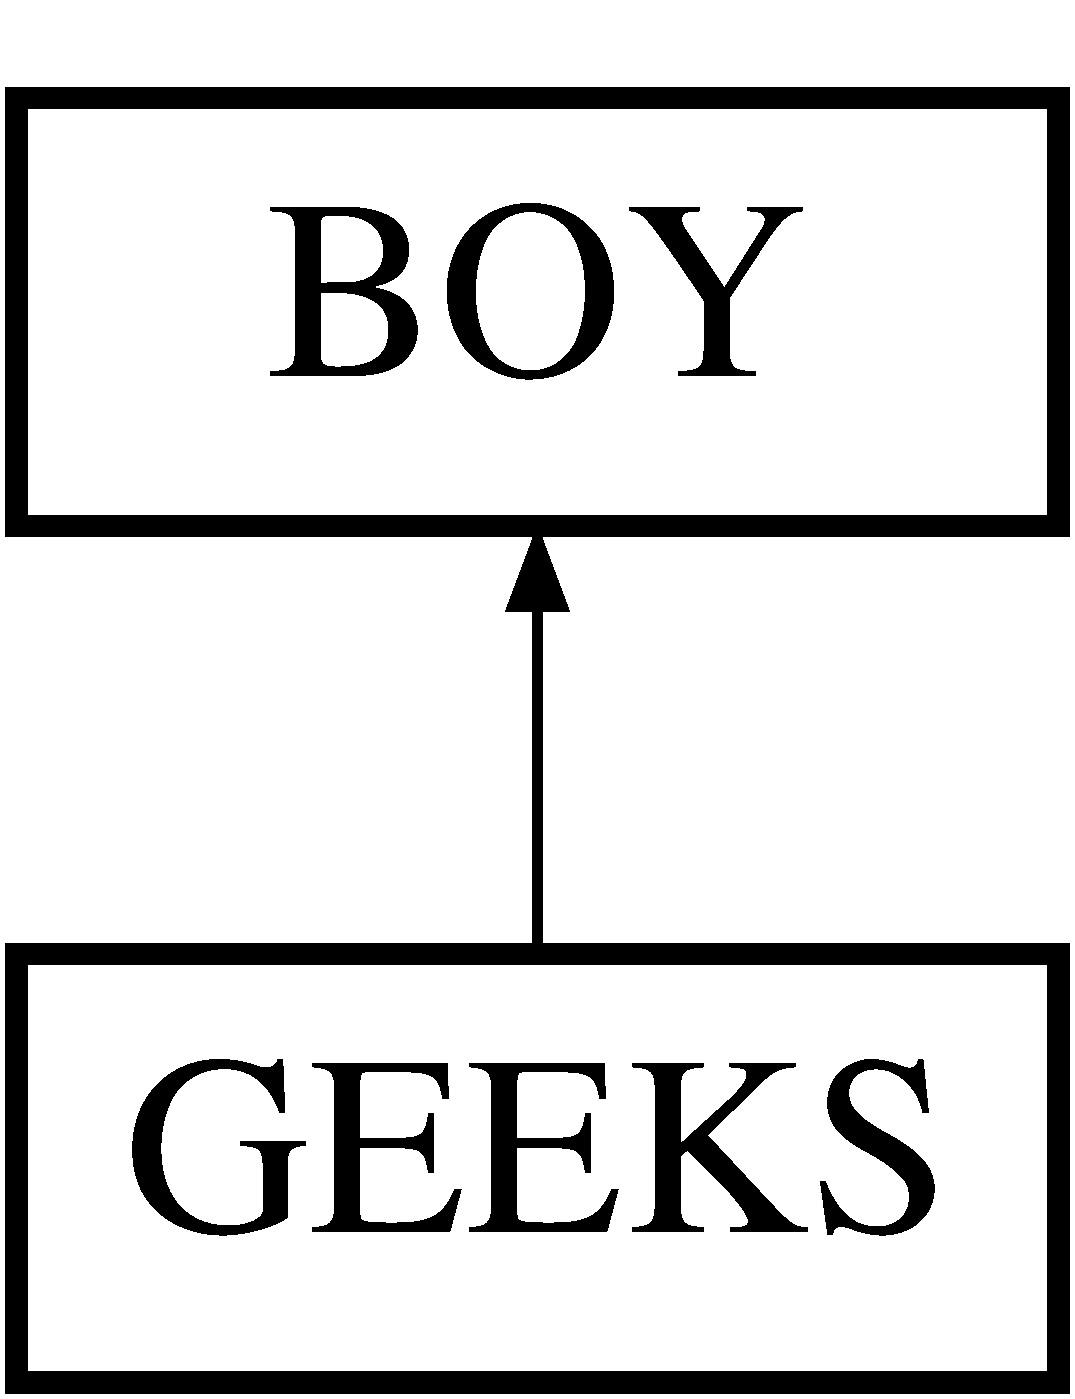
\includegraphics[height=2.000000cm]{classGEEKS}
\end{center}
\end{figure}
\subsection*{Public Member Functions}
\begin{DoxyCompactItemize}
\item 
\mbox{\Hypertarget{classGEEKS_a6425e88aeb8a0fb7e7502bf2b8a9f037}\label{classGEEKS_a6425e88aeb8a0fb7e7502bf2b8a9f037}} 
double \hyperlink{classGEEKS_a6425e88aeb8a0fb7e7502bf2b8a9f037}{cal\+\_\+happ} (double girl\+\_\+happ)
\begin{DoxyCompactList}\small\item\em child class of \hyperlink{classBOY}{B\+OY} class \end{DoxyCompactList}\end{DoxyCompactItemize}
\subsection*{Additional Inherited Members}


The documentation for this class was generated from the following file\+:\begin{DoxyCompactItemize}
\item 
G\+E\+E\+K\+S.\+h\end{DoxyCompactItemize}

\hypertarget{classGENEROUS}{}\section{G\+E\+N\+E\+R\+O\+US Class Reference}
\label{classGENEROUS}\index{G\+E\+N\+E\+R\+O\+US@{G\+E\+N\+E\+R\+O\+US}}


class name \hyperlink{classGENEROUS}{G\+E\+N\+E\+R\+O\+US}  




{\ttfamily \#include $<$G\+E\+N\+E\+R\+O\+U\+S.\+h$>$}

Inheritance diagram for G\+E\+N\+E\+R\+O\+US\+:\begin{figure}[H]
\begin{center}
\leavevmode
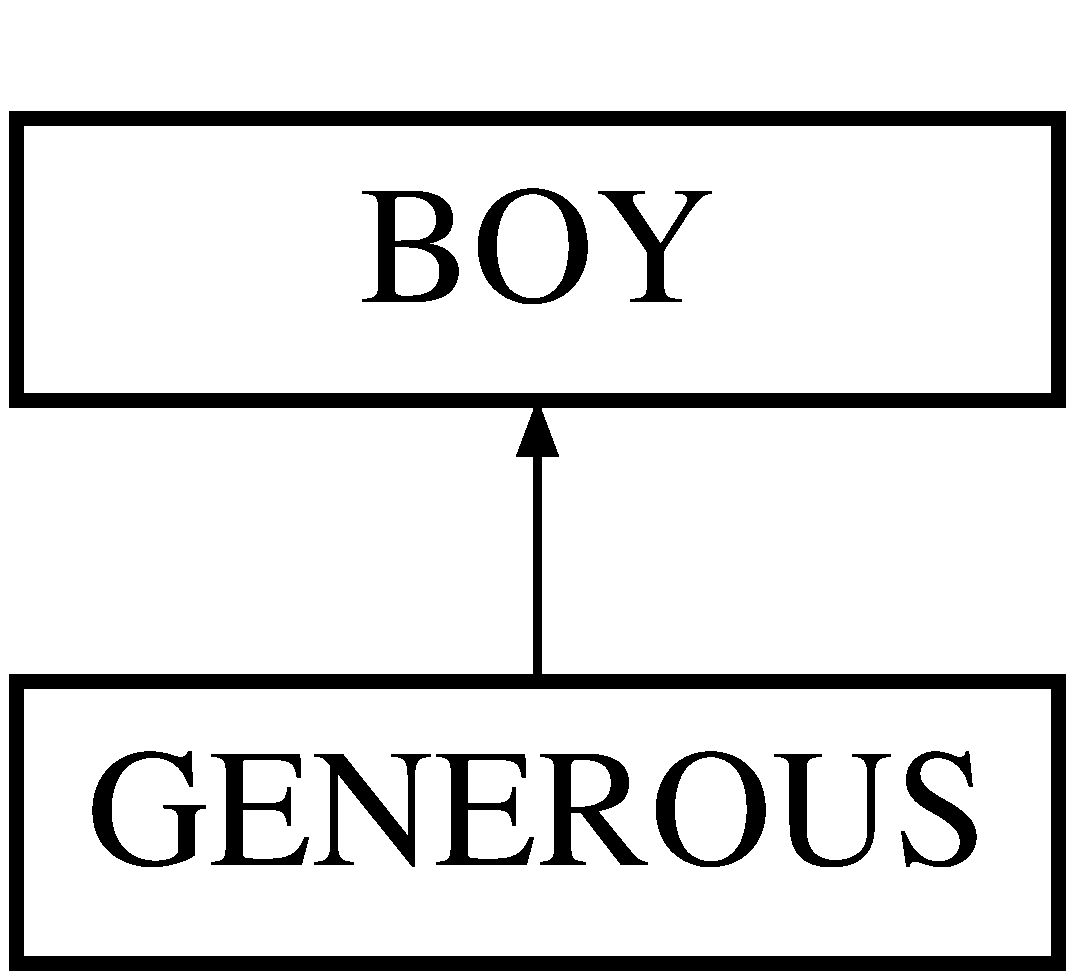
\includegraphics[height=2.000000cm]{classGENEROUS}
\end{center}
\end{figure}
\subsection*{Public Member Functions}
\begin{DoxyCompactItemize}
\item 
double \hyperlink{classGENEROUS_afbeff7b10bbd75135cca3485cb50a537}{cal\+\_\+happ} (double girl\+\_\+happ)
\begin{DoxyCompactList}\small\item\em child class of \hyperlink{classBOY}{B\+OY} class \end{DoxyCompactList}\end{DoxyCompactItemize}
\subsection*{Additional Inherited Members}


\subsection{Detailed Description}
class name \hyperlink{classGENEROUS}{G\+E\+N\+E\+R\+O\+US} 

\subsection{Member Function Documentation}
\mbox{\Hypertarget{classGENEROUS_afbeff7b10bbd75135cca3485cb50a537}\label{classGENEROUS_afbeff7b10bbd75135cca3485cb50a537}} 
\index{G\+E\+N\+E\+R\+O\+US@{G\+E\+N\+E\+R\+O\+US}!cal\+\_\+happ@{cal\+\_\+happ}}
\index{cal\+\_\+happ@{cal\+\_\+happ}!G\+E\+N\+E\+R\+O\+US@{G\+E\+N\+E\+R\+O\+US}}
\subsubsection{\texorpdfstring{cal\+\_\+happ()}{cal\_happ()}}
{\footnotesize\ttfamily double G\+E\+N\+E\+R\+O\+U\+S\+::cal\+\_\+happ (\begin{DoxyParamCaption}\item[{double}]{girl\+\_\+happ }\end{DoxyParamCaption})\hspace{0.3cm}{\ttfamily [inline]}}



child class of \hyperlink{classBOY}{B\+OY} class 

calculates happiness 

The documentation for this class was generated from the following file\+:\begin{DoxyCompactItemize}
\item 
G\+E\+N\+E\+R\+O\+U\+S.\+h\end{DoxyCompactItemize}

\hypertarget{classGIFT}{}\section{G\+I\+FT Class Reference}
\label{classGIFT}\index{G\+I\+FT@{G\+I\+FT}}
\subsection*{Public Attributes}
\begin{DoxyCompactItemize}
\item 
\mbox{\Hypertarget{classGIFT_af2e9da1e8ab6b8aedbce10cfd26d14e4}\label{classGIFT_af2e9da1e8ab6b8aedbce10cfd26d14e4}} 
int {\bfseries price}
\item 
\mbox{\Hypertarget{classGIFT_a4147df96f0f8610af3c78df7c5986640}\label{classGIFT_a4147df96f0f8610af3c78df7c5986640}} 
int \hyperlink{classGIFT_a4147df96f0f8610af3c78df7c5986640}{value}
\begin{DoxyCompactList}\small\item\em price of gift \end{DoxyCompactList}\item 
\mbox{\Hypertarget{classGIFT_acc9e2848b7ac3250c279453d1c49641a}\label{classGIFT_acc9e2848b7ac3250c279453d1c49641a}} 
char \hyperlink{classGIFT_acc9e2848b7ac3250c279453d1c49641a}{type} \mbox{[}10\mbox{]}
\begin{DoxyCompactList}\small\item\em value of gift \end{DoxyCompactList}\end{DoxyCompactItemize}


The documentation for this class was generated from the following files\+:\begin{DoxyCompactItemize}
\item 
ppl\+Q2.\+cpp\item 
G\+I\+F\+T.\+h\end{DoxyCompactItemize}

\hypertarget{classGIRL}{}\section{G\+I\+RL Class Reference}
\label{classGIRL}\index{G\+I\+RL@{G\+I\+RL}}
Inheritance diagram for G\+I\+RL\+:\begin{figure}[H]
\begin{center}
\leavevmode
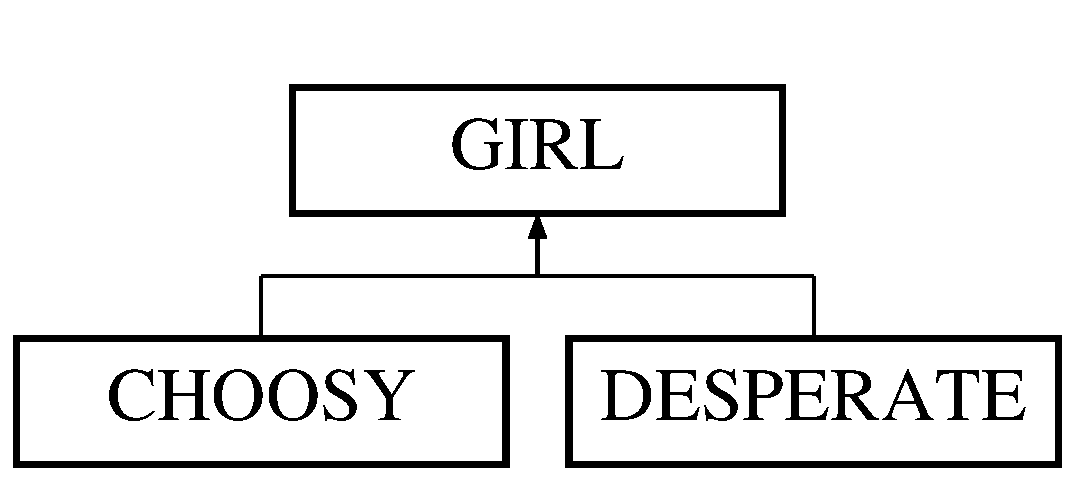
\includegraphics[height=2.000000cm]{classGIRL}
\end{center}
\end{figure}
\subsection*{Public Attributes}
\begin{DoxyCompactItemize}
\item 
\mbox{\Hypertarget{classGIRL_a3a2d0315c5af8dff6c40c85a178d8dc3}\label{classGIRL_a3a2d0315c5af8dff6c40c85a178d8dc3}} 
char {\bfseries name} \mbox{[}10\mbox{]}
\item 
\mbox{\Hypertarget{classGIRL_ad318803047f459499d8ca04e273ffeeb}\label{classGIRL_ad318803047f459499d8ca04e273ffeeb}} 
int {\bfseries attract}
\item 
\mbox{\Hypertarget{classGIRL_a5a923dc63a6d09356099489d4c7dfbde}\label{classGIRL_a5a923dc63a6d09356099489d4c7dfbde}} 
int \hyperlink{classGIRL_a5a923dc63a6d09356099489d4c7dfbde}{budget}
\begin{DoxyCompactList}\small\item\em attractiveness \end{DoxyCompactList}\item 
\mbox{\Hypertarget{classGIRL_aa6da8c4ab9f34e119e8d572edeb404a5}\label{classGIRL_aa6da8c4ab9f34e119e8d572edeb404a5}} 
int \hyperlink{classGIRL_aa6da8c4ab9f34e119e8d572edeb404a5}{int\+\_\+level}
\begin{DoxyCompactList}\small\item\em maintenance cost \end{DoxyCompactList}\item 
\mbox{\Hypertarget{classGIRL_a7c4d97852a7d44914fec313f6466d4b2}\label{classGIRL_a7c4d97852a7d44914fec313f6466d4b2}} 
char \hyperlink{classGIRL_a7c4d97852a7d44914fec313f6466d4b2}{type} \mbox{[}10\mbox{]}
\begin{DoxyCompactList}\small\item\em status \end{DoxyCompactList}\item 
\mbox{\Hypertarget{classGIRL_aef64b91193f89b0500a984c0433bfdd8}\label{classGIRL_aef64b91193f89b0500a984c0433bfdd8}} 
double \hyperlink{classGIRL_aef64b91193f89b0500a984c0433bfdd8}{happ}
\begin{DoxyCompactList}\small\item\em intelligence level \end{DoxyCompactList}\item 
\mbox{\Hypertarget{classGIRL_a27478c12737eefcdaadc760b33876772}\label{classGIRL_a27478c12737eefcdaadc760b33876772}} 
char \hyperlink{classGIRL_a27478c12737eefcdaadc760b33876772}{status} \mbox{[}10\mbox{]}
\begin{DoxyCompactList}\small\item\em happiness \end{DoxyCompactList}\end{DoxyCompactItemize}


The documentation for this class was generated from the following files\+:\begin{DoxyCompactItemize}
\item 
ppl\+Q2.\+cpp\item 
G\+I\+R\+L.\+h\end{DoxyCompactItemize}

\hypertarget{classMISER}{}\section{M\+I\+S\+ER Class Reference}
\label{classMISER}\index{M\+I\+S\+ER@{M\+I\+S\+ER}}
Inheritance diagram for M\+I\+S\+ER\+:\begin{figure}[H]
\begin{center}
\leavevmode
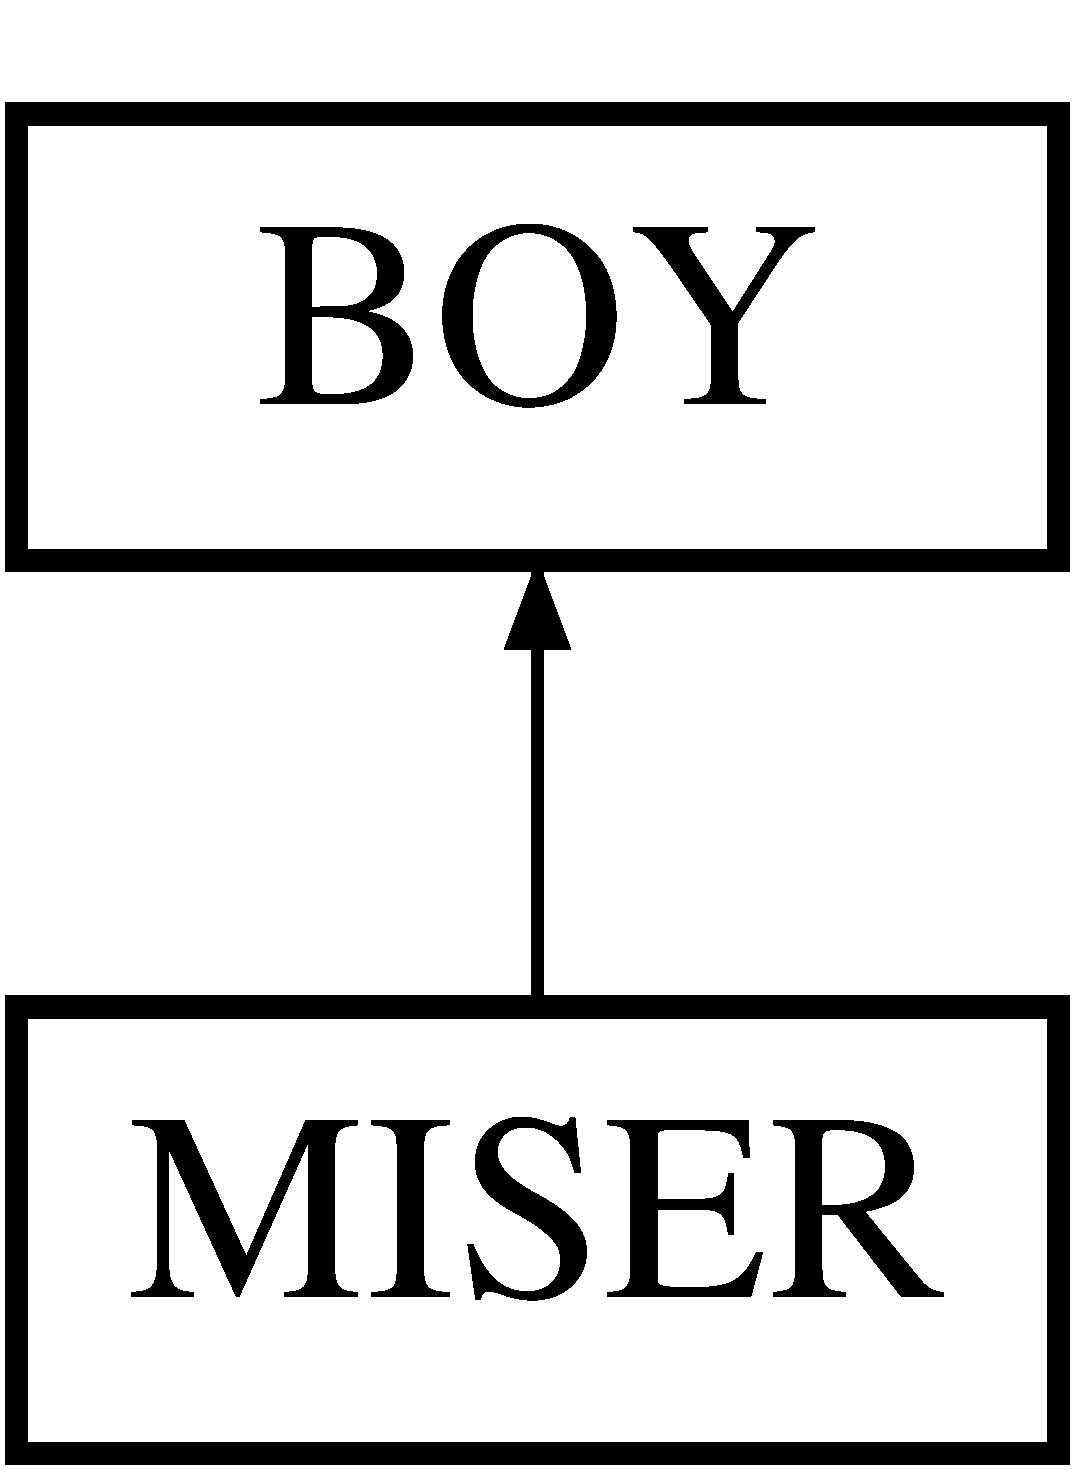
\includegraphics[height=2.000000cm]{classMISER}
\end{center}
\end{figure}
\subsection*{Public Member Functions}
\begin{DoxyCompactItemize}
\item 
double \hyperlink{classMISER_a178be2918344f7c56b1d64b531053cd1}{cal\+\_\+happ} (double girl\+\_\+happ)
\begin{DoxyCompactList}\small\item\em child class of \hyperlink{classBOY}{B\+OY} class \end{DoxyCompactList}\end{DoxyCompactItemize}
\subsection*{Additional Inherited Members}


\subsection{Member Function Documentation}
\mbox{\Hypertarget{classMISER_a178be2918344f7c56b1d64b531053cd1}\label{classMISER_a178be2918344f7c56b1d64b531053cd1}} 
\index{M\+I\+S\+ER@{M\+I\+S\+ER}!cal\+\_\+happ@{cal\+\_\+happ}}
\index{cal\+\_\+happ@{cal\+\_\+happ}!M\+I\+S\+ER@{M\+I\+S\+ER}}
\subsubsection{\texorpdfstring{cal\+\_\+happ()}{cal\_happ()}}
{\footnotesize\ttfamily double M\+I\+S\+E\+R\+::cal\+\_\+happ (\begin{DoxyParamCaption}\item[{double}]{girl\+\_\+happ }\end{DoxyParamCaption})\hspace{0.3cm}{\ttfamily [inline]}}



child class of \hyperlink{classBOY}{B\+OY} class 

calculates happiness 

The documentation for this class was generated from the following file\+:\begin{DoxyCompactItemize}
\item 
M\+I\+S\+E\+R.\+h\end{DoxyCompactItemize}

%--- End generated contents ---

% Index
\backmatter
\newpage
\phantomsection
\clearemptydoublepage
\addcontentsline{toc}{chapter}{Index}
\printindex

\end{document}
